%----------------------------------------------------------------------------------------
%       PACKAGES AND OTHER DOCUMENT CONFIGURATIONS
%----------------------------------------------------------------------------------------
\documentclass[paper=letter, fontsize=12pt]{article}
\usepackage[english]{babel} % English language/hyphenation
\usepackage{amsmath,amsfonts,amsthm} % Math packages
\usepackage[utf8]{inputenc}
\usepackage{lipsum} % Package to generate dummy text throughout this template
\usepackage{graphicx} 
\usepackage{caption}
\usepackage{subcaption}
\usepackage{listings}
\usepackage[sc]{mathpazo} % Use the Palatino font
\linespread{1.05} % Line spacing - Palatino needs more space between lines
\usepackage{microtype} % Slightly tweak font spacing for aesthetics
\usepackage[hmarginratio=1:1,top=32mm,columnsep=20pt]{geometry} % Document margins
\usepackage{multicol} % Used for the two-column layout of the document
%\usepackage[hang, small,labelfont=bf,up,textfont=it,up]{caption} % Custom captions under/above floats in tables or figures
\usepackage{booktabs} % Horizontal rules in tables
\usepackage{float} % Required for tables and figures in the multi-column environment - they need to be placed in specific locations with the [H] (e.g. \begin{table}[H])
\usepackage[hidelinks=true]{hyperref} % For hyperlinks in the PDF
\usepackage{lettrine} % The lettrine is the first enlarged letter at the beginning of the text
\usepackage{paralist} % Used for the compactitem environment which makes bullet points with less space between them
\usepackage{abstract} % Allows abstract customization
\renewcommand{\abstractnamefont}{\normalfont\bfseries} % Set the "Abstract" text to bold
\renewcommand{\abstracttextfont}{\normalfont\small\itshape} % Set the abstract itself to small italic text
\usepackage{titlesec} % Allows customization of titles
\usepackage{marvosym}
\usepackage{array}
\usepackage{csquotes}
\usepackage{bytefield}
\usepackage{xcolor}
\usepackage{pifont}
\usepackage[underline=true]{pgf-umlsd}
\usepackage{pdflscape}
\usepackage{cite}
\usepackage{wasysym}
\usepackage{csquotes}
\usepackage[export]{adjustbox}
\usepackage{moeptikz}
\usepackage[separate-uncertainty=true,quotient-mode=fraction]{siunitx}
\usepackage{makecell}
\usepackage[T1]{fontenc}
\usepackage{pgfgantt-custom}
\sisetup{exponent-product = \cdot, output-product = \cdot}

\usetikzlibrary{calc}

\titleformat{\section}[block]{\large}{\thesection.}{1em}{} % Change the look of the section titles
\titleformat{\subsection}[block]{\large}{\thesubsection.}{1em}{} % Change the look of the subsection titles
\newcommand{\horrule}[1]{\rule{\linewidth}{#1}} % Create horizontal rule command with 1 argument of height
\usepackage{fancyhdr} % Headers and footers
\pagestyle{fancy} % All pages have headers and footers
\fancyhead{} % Blank out the default header
\fancyfoot{} % Blank out the default footer

\fancyhead[C]{Technische Universität München $\bullet\enskip$\today$\enskip\bullet$ Group 17 }

\fancyfoot[RO,LE]{\thepage} % Custom footer text

% COLOR DEFINITIONS
\definecolor{darkestBrew}{RGB}{191,80,29}
\definecolor{darkBrew}{RGB}{230,85,13}
\definecolor{mediumBrew}{RGB}{253,141,60}
\definecolor{lightBrew}{RGB}{253,190,133}
\definecolor{lightestBrew}{RGB}{254,237,222}


\DeclareUnicodeCharacter{2603}{\snowman}

%----------------------------------------------------------------------------------------
%       TITLE SECTION
%----------------------------------------------------------------------------------------
\title{\vspace{-15mm}\fontsize{24pt}{10pt}\selectfont\textbf{Final Report: \\Onion Module}} % Article title
\author{
\large
{\textsc{Marko Dorfhuber (03658730) $\quad$ \Letter marko.dorfhuber@tum.de}}\\[2mm]
{\textsc{Christoph Rudolf (03662116) $\quad$ \Letter christoph.rudolf@tum.de}}\\[2mm]
%\thanks{A thank you or further information}\\ % Your name
%\normalsize \href{mailto:marco.torres.810@gmail.com}{marco.torres.810@gmail.com}\\[2mm] % Your email address
}
\date{}

\input{listings_def.lst}

%----------------------------------------------------------------------------------------
\begin{document}
\maketitle % Insert title
\thispagestyle{fancy} % All pages have headers and footers

\section{Overview over the architecture}
This section aims to give an overview over the basic architecture and components of the final implementation of the Onion module.
The interim report gave an abstract overview over the environment of the Onion Module, making clear that its central role in the Voidphone application requires the module to have many interfaces. Figure~\ref{fig:architecture} shows a more detailed representation of the final design. The figure can be seen as the inner workings of the \emph{Onion Module} component depicted in the component diagram of the interim report (see Figure~1 of the interim report). 

Each interface the Onion module has towards another module is managed by a respective interface class. Common base classes like for example an abstract \texttt{TcpClientInterface} for Authentication and RPS are used to encapsulate shared functionality among these interface classes. The common basis for all elements with networking code is the \textbf{Netty}\footnote{\url{http://netty.io/}} framework, an asynchronous event-driven network application framework based on Java's NIO. 

Each of the interfaces references a parser specific for the data that is expected on this interface. The parser is given the raw bytes which is received by the interface and returns a serialized message instance or a parsing error. The parsers are also used by the refercing modules to build the message types they are sending. All references between components are setup via \emph{Depedency Injection} using Google's \textbf{Guice} framework.

\usetikzlibrary{positioning,shapes.misc}
\tikzstyle{orchestrator} = [rectangle, draw=black, text=white, fill=darkestBrew, rounded corners=15pt, text width=7.5em, minimum height=7.5em, minimum width=7mm]
\tikzstyle{interface} = [rectangle, draw=black, text=black, fill=mediumBrew, rounded corners=5pt, text centered, text width=6.5em, minimum height=4em, minimum width=6mm]
\tikzstyle{config} = [rectangle, draw=black, dashed, text=black, fill=lightBrew, rounded corners=5pt, text centered, text width=6.5em, minimum height=4em, minimum width=6mm]
\tikzstyle{parser} = [rectangle, draw=black, dashed, text=black, fill=lightestBrew, rounded corners=3pt, text centered, text width=6.5em, minimum height=2.5em, minimum width=6.5mm]
\begin{figure}[ht]
\resizebox{\textwidth}{!}{\begin{tikzpicture}[x=1mm,y=1mm, >=latex, ->]
    \node[orchestrator] (orchestrator) {\hspace{1.5mm}\large{Orchestrator} \\ \vspace{2mm} \hspace{0.6mm}\scriptsize{$\bullet$ handles rounds} \raisebox{-0.7ex}{\Large{\clock}} \\ \hspace{0.6mm}\scriptsize{$\bullet$ holds state}};

    % Interface elements
    \node[interface, left of=orchestrator, node distance=14em] (onionInterface) {Onion P2P \\ Interface};
    \node[interface, right of=orchestrator, node distance=14em] (apiInterface) {Onion API \\ Interface};
    \node[interface, below of=onionInterface, node distance=9em] (authInterface) {Onion \\ Authentication \\ Interface};
    \node[interface, right of=authInterface, node distance=21em] (rpsInterface) {RPS \\ Interface};

    \node[config, above of=orchestrator, node distance=9em] (configProvider) {Configuration \\ Provider};

    % Connections
    \draw [-{latex[scale=1.2]}] (orchestrator) edge (configProvider);
    \draw [-{latex[scale=1.2]}] (orchestrator) edge (rpsInterface);
    \draw [{latex[scale=1.2]}-{latex[scale=1.2]}] (orchestrator) edge node [text width=20mm, midway, align=center] {\footnotesize{reference and callback}} (onionInterface);
    \draw [{latex[scale=1.2]}-{latex[scale=1.2]}] (orchestrator) edge node [text width=20mm, midway, align=center] {\footnotesize{reference and callback}} (apiInterface);
    \draw [-{latex[scale=1.2]}] (onionInterface) edge (authInterface);

    % Parser
    \node[parser, above of=onionInterface, node distance=3.2em] (onionInterface) {Parser};
    \node[parser, above of=apiInterface, node distance=3.2em] (apiInterface) {Parser};
    \node[parser, below of=rpsInterface, node distance=3.2em] (rpsParser) {Parser};
    \node[parser, below of=authInterface, node distance=3.2em] (rpsParser) {Parser};

\end{tikzpicture}}
    \caption{Architecture overview of the final implementation.}
    \label{fig:architecture}
\end{figure}


\begin{description}
    \item [The Orchestrator] acts as a starting point for the module and manages a total of three interfaces (\texttt{RPS Interface}, \texttt{Onion API Interface}, \texttt{Onion P2P Interface}). It's job is to issue the start of rounds and to manage data flow between interfaces. For this, the \texttt{Orchestrator} has references and callbacks towards interfaces. In case of an event on one interface that affects another one, an approriate transfer is done. An example would be that the CM/UI module wants to build a new tunnel which requires the sampling of hops via the \texttt{RPS Interface} as well as the tunnel build itself by the \texttt{Onion P2P interface}. The \texttt{Orchestrator} also references the \texttt{Configuration Provider} which reads the configuration file and parses it to provide the given data to all modules.

    \item [The Onion API Interface] acts as a TCP server for a connecting UI/CM module. It is able to handle all messages specified as Onion API messages in the specificationn~\cite{spec}.
    A callback connects the interface to the \texttt{Orchestrator} and notifies it of incoming requests.

    \item [The RPS Interface] is the simplest interface, acting as a TCP client towards the RPS module. It only provides one method to query a random peer (using the \texttt{RPS QUERY} message type) which encapsulates the call to the other module.

    \item [The Onion P2P Interface] is in charge of managing the peer-to-peer connections (tunnels) to other modules. It acts as a combined UDP server and client. Its parser handles our custom P2P protocol (see Section~\ref{sec:protocol}). The \texttt{Onion Authentication Interface}, a client to the Authentication module, is referenced directly. This accounts for the fact that both modules are strongly connected, even being combined into one in the past. The P2P interfaces is the only module who uses the \texttt{Onion Authentication Interface} and needs to call its functionality frequently during tunnel operations which do not trigger any callback to the \texttt{Orchestrator}. This way, the \texttt{Orchestrator} can simply issue a tunnel to be build, select the random peers and is not required to handle roundtrips to the authentication module for every encryption happening as a result.

    \item [Data structures and identifiers:] The application has a set of central data structures used to store its state. The major ones are collections of tunnels started by the running peer as initiator (\texttt{startedTunnels}), tunnels that this peer acts as an endpoint to (\texttt{incomingTunnels}) and states for this peer's role as an intermediate hop (\texttt{intermediateSegments}). The collections are created by the \texttt{Orchestrator} and also accessible by the \texttt{Onion P2P Interface}. 
    From the perspective of the application, a tunnel is an object with a tunnel identifier and a list of tunnel segments. The segments have precise information about adjecent hops (address and port). A segment created for each hop of a tunnel, describing the state between the tunnel initiator and this hop. Therefore, a segment does also now about the session it belongs to and is identified by a \emph{local identifier}. In a peers role as an intermediate hop, each tunnel segment gets a matching counterpart segment assigned. With this, a peer is able to match forwarding of data with a certain LID in both ways through the tunnel. Each time, he has to write the corresponding LID expected by the next peer inside the message header. It is noteworthy that for a peer's role as intermediate hop, we only store tunnel segments (not whole tunnels) as an additional grouping by tunnel ID, has no relevance for this peer. Tunnel IDs, and therefore whole tunnel instances, are only stored for tunnels a peer started and the ones he received as an endpoint, as these are scenarios in which the peer has to report to its respective UI/CM module stating a tunnel ID. 

    The \textbf{local identifiers (LIDs)} have been introduced in the interim report and, as we noticed during the lectures on TOR, correspond to the circuit IDs in TOR. They are valid between the initiator and a specific hop of a tunnel. The LID allows an intermediate peer to match an incoming packet to a session and a tunnel-specific next hop for forwarding. Figure~\ref{fig:lids} taken from our interim report visualize the concept and the validity of the identifiers in an Onion tunnel with two intermediate hops.

    \begin{figure}[ht]
    \centering
    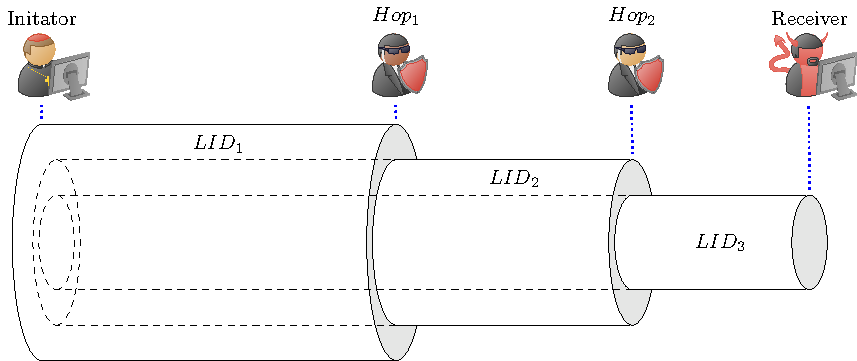
\includegraphics[width=.94\textwidth,right]{images/lids.pdf}
    \caption{Structure of a tunnel and validity of the local tunnel identifiers (LIDs).}
    \label{fig:lids}
    \end{figure}
\end{description}

\section{Final Onion P2P protocol}
\label{sec:protocol}

The protocol proposed in the interim report underwent minor improvements due to specification changes regarding the fixed size of packets. With new message types towards the authentication module, we are now able to maintain a fixed message size during onion layer encryption at each hop. With the lectures on TOR's onion protocol that happened shortly after the interim report's submission and the changes to the specification, we were able to refine our protocol.

This section describes the final message types for the Onion P2P protocol and the purpose of each. Not all message types underwent changes, however, this section still includes them to provide a complete replacement to the interim report. In order to maintain consistency with the inter-module protocols defined by the specification, each message type starts with a fixed four byte header that includes the message size and its type. We additionally specified a 128 bit local identifier (LID) to follow for every type.

\subsection{Onion Tunnel Init}

This messages indicates the beginning of a new tunnel segment and is created after the \texttt{Onion API Interfaces} 
receives the ONION TUNNEL BUILD message from its client CM/UI module or choses to create a tunnel
for cover traffic on its own. Messages of this type are sent iteratively by the tunnel initiator to
the peers he choses to be part of the tunnel. Eachg encrypted depending on how far the tunnel is already setup. 
It is used to transmit the first handshake data given by the Onion Authentication module. \\

\begin{bytefield}[bitwidth=1.1em]{32}
    \bitheader{0,7,8,15,16,23,24,31} \\
    \bitbox{16}{size} & \bitbox{16}{\texttt{ONION TUNNEL INIT} = 595} \\ 
    \wordbox{4}{local tunnel identifier (LID)} \\ 
    \wordbox[tlr]{2}{handshake payload from \texttt{AUTH SESSION HS1}} \\
    \skippedwords \\
    \wordbox[blr]{1}{}
\end{bytefield}

\subsection{Onion Tunnel Accept}

This messages is the expected response to the \texttt{ONION TUNNEL INIT} message. It contains the local
tunnel identifier specified in the matching \texttt{ONION TUNNEL INIT} and forwards the data this peer
received from its Onion Authentication module in \texttt{AUTH SESSION HS2}. 
This finishes the session establishment and allows for a subsequent encryption of 
messages between the initiator and the sending peer. \\

\begin{bytefield}[bitwidth=1.1em]{32}
    \bitheader{0,7,8,15,16,23,24,31} \\
    \bitbox{16}{size} & \bitbox{16}{\texttt{ONION TUNNEL ACCEPT} = 596} \\ 
    \wordbox{4}{local tunnel identifier (LID)} \\ 
    \wordbox[tlr]{2}{handshake payload from \texttt{AUTH SESSION HS2}} \\
    \skippedwords \\
    \wordbox[blr]{1}{}
\end{bytefield}

\subsection{Onion Tunnel Relay}

The relay message is used to instruct a host that is already part of the tunnel, to send data to a new
host currently outside of the tunnel. This instruction can already be encrypted with the session
keys established so far. With this message, the forwarding host is also instructed to assign the new
host as its successor for this tunnel segment. This message is necessary for tunnel building when
the currently last hop expands the tunnel with a new hop.
The message includes the address and port the new peer is reachable on. An additional bit \texttt{V} defines the
usage of IPv4 (= 0) or IPv6 (= 1). Subsequently, the message includes the local identifier matching
the connection from the initiator to the new peer. This LID allows the receiver of this message to
create a mapping for further forwarding. The received data is sent to the specified peer. \\

\begin{bytefield}[bitwidth=1.1em]{32}
    \bitheader{0,7,8,15,16,23,24,31} \\
    \bitbox{16}{size} & \bitbox{16}{\texttt{ONION TUNNEL RELAY} = 597} \\
    \wordbox{4}{local tunnel identifier (LID$_1$) \\ between the initiator and the receiver} \\ 
	\bitbox{16}{port} & \bitbox{1}{V} & \bitbox{15}{reserved} \\
    \wordbox{1}{address (i.\,e. IP address) of the host to forward to} \\
    \wordbox{4}{local tunnel identifier (LID$_2$) \\ between the initiator and the new hop} \\ 
    \wordbox[tlr]{2}{data for the new hop (e.\,g. a \texttt{ONION TUNNEL INIT} message)} \\
    \skippedwords \\
    \wordbox[blr]{1}{} 
\end{bytefield}

\subsection{Onion Tunnel Transport}
The \texttt{ONION TUNNEL TRANSPORT} message is used to securely transmit arbitrary data over an already established tunnel. 
Therefore, it can possibly contain any other message type as data and is maintaining a fixed length in all cases in order to provide a defense against an attacker using
traffic analysis to gain intel on anonymous communications.

Our calculation provided with the interim report regarding the size of data such a message has to be able to contain, still holds. For this, we considered average human speech in combination with bitrates of common VoiP codecs. This was to make sure a single lost packet does not contain a crucial amount of voice data which would hurt the quality of the phone call. However, with the new changes introduced to this message type, we do not rely on a padding scheme like PKCS7~\#7 any longer. Instead, the size of the inner real data is given explicitly by its length field and random padding data can be stripped, just like in TOR.

Every time an arbitrary other Onion P2P message type is to be encapsulated the new procedure for transport messages is:
\begin{enumerate}
    \item The inner packet has to have a maximum size of 508 byte (including its header, larger voice data is fragmented).
    \item A fixed four byte magic string is added (with that a peer can quickly check if he is the receiver).
    \item The resulting 512 byte block is encrypted with either \texttt{AUTH LAYER ENCRYPT} or \texttt{AUTH CIPHER ENCRYPT} and its E flag set to 0
    \item The resulting cipher data is put into a \texttt{ONION TUNNEL TRANSPORT} message after the LID.
    
    \emph{Note: the cipher can be larger than 512 byte due to an overhead (c) the authentication module might produce due to IVs oder MACs. However, further en- and decryption is designed to keep this size constant. With a fixed plain input length of 512 byte to the authentication module's encryption mechanism, we are guaranteed to have a fixed message size.}
    \item Receivers that decrypt the message once, determine if they are left with plain data by checking the "PtoP" string.
    \item Random padding can be stripped by parsing the length field of the contained message type. \\
\end{enumerate}

\begin{bytefield}[bitwidth=1.1em]{32}
    \bitheader{0,7,8,15,16,23,24,31} \\
    \bitbox{16}{size = 536 + c} & \bitbox{16}{\texttt{ONION TUNNEL TRANSPORT} = 598} \\ 
    \wordbox{4}{local tunnel identifier (LID$_1$) \\ between the initiator and the receiver} \\
    \begin{rightwordgroup}{encrypted \\ and padded \\ with the \\ session key \\ belonging \\ to LID$_1$. \\ Encrypted size: \\ \SI{512}{byte} + c}
        \bitbox{32}{"PtoP"} \\
        \wordbox[tlr]{2}{data to be forwarded} \\
        \skippedwords \\
        \wordbox[blr]{1}{}
    \end{rightwordgroup} \\
\end{bytefield}

\subsection{Onion Tunnel Established}
\label{sec:protocol:established}

The \texttt{ONION TUNNEL ESTABLISHED} message type is used to notify a peer that it is the final hop in a tunnel. This is necessary as peers have to send a
\texttt{ONION TUNNEL INCOMING} message to their UI/CM in this case. Without a separate message type, a peer is unable to know about its role as an endpoint, as an extension of the tunnel towards a new peer can happen at any time. An alternative to this message type would be to treat the first incoming voice data as a signal of being the final hop.
However, a called peer might also want to start sending voice data before receiving any.
Section~\ref{sec:function:build} displays how this message is used during the tunnel building phase.

\begin{bytefield}[bitwidth=1.1em]{32}
    \bitheader{0,7,8,15,16,23,24,31} \\
    \bitbox{16}{size} & \bitbox{16}{\texttt{ONION TUNNEL ESTABLISHED} = 593} \\ 
    \wordbox{4}{local tunnel identifier (LID$_{new}$) \\ between the sender and receiver} \\
\end{bytefield}

The \texttt{ONION TUNNEL ESTABLISHED} does also come in a second version including two local identifiers (additional, optional LID is marked in gray). This is used when we transparently switch over an ongoing call to a fresh tunnel. To do so, this message type indicates a replacement from the old to the new identifier to be mapped to an existing call. Section~\ref{sec:function:switch} displays how this message is used during tunnel switching. \\

\begin{bytefield}[bitwidth=1.1em]{32}
    \bitheader{0,7,8,15,16,23,24,31} \\
    \bitbox{16}{size} & \bitbox{16}{\texttt{ONION TUNNEL ESTABLISHED} = 593} \\ 
    \wordbox{4}{\textbf{new} local tunnel identifier (LID$_{new}$) \\ between the sender and receiver} \\
    \wordbox{4}{\textbf{old} local tunnel identifier (LID$_{old}$) \\ between the sender and receiver} \\
\end{bytefield}

\subsection{Onion Tunnel Voice}
This message type is used to transmit voice data over an established tunnel. It is always encrypted inside a \texttt{ONION TUNNEL TRANSPORT} message.
A peer retrieving this message from encrypting a transport message type expects to be a tunnel endpoint regarding the given LID.
The included voice data can then be forwarded to the UI/CM module with the tunnel ID associated to the included LID in the peer's state. \\

\begin{bytefield}[bitwidth=1.1em]{32}
    \bitheader{0,7,8,15,16,23,24,31} \\
    \bitbox{16}{size} & \bitbox{16}{\texttt{ONION TUNNEL VOICE} = 594} \\ 
    \wordbox{4}{local tunnel identifier (LID$_1$) \\ between the sender and receiver} \\
    \wordbox[tlr]{2}{raw voice data} \\
    \skippedwords \\
    \wordbox[blr]{1}{} 
\end{bytefield}


\subsection{Onion Tunnel Teardown}

The teardown process of a tunnel can only be issued by its originator. This is necessary because a
tunnel has to be teared down beginning from very the last hop and only the originator can send
an encrypted teardown message through the whole tunnel. Unencrypted and therefore unauthenticated tear downs would
introduce a huge weakness to denial of service attacks on existing tunnels. 
To tear down a tunnel, this message is iteratively sent through the tunnel starting from the last hop.

If the endpoint of a tunnel is instructed to tear down a tunnel by its UI/CM module, he uses the same message type.
This then propagates through the tunnel until it reaches the hop that identifies itself as initiator. 
The initiator is then able to destroy the tunnel as described (see sequence in Section~\ref{sec:function:teardown}). \\

\begin{bytefield}[bitwidth=1.1em]{32}
    \bitheader{0,7,8,15,16,23,24,31} \\
    \bitbox{16}{size} & \bitbox{16}{\texttt{ONION TUNNEL TEARDOWN} = 599} \\ 
    \wordbox{4}{local tunnel identifier (LID$_1$) \\ between the sender and receiver} \\
\end{bytefield}

\section{Functioning}
This section describes how the individual steps of tunnel handling (build, usage, teardown, transparent switching, cleanup) function in the final implementation. For each step, a protocol sequence with only one intermediate hop is given. This is only done due to the limited space on a portrait oriented page. Additional intermediate hops do not add any additional behavior, and only lead to more forwarding and layer encryption.
%however, a full sequence diagram with two hops is given at the end of this chapter as Figure~\ref{fig:sequence}. 
The identical headers with size and type are abbreviated by a shorthand for the respective message types. The also identical local identifiers of each message type are specified to make clear which LID is used. 

\textbf{Note that data inside a \texttt{transport} message after the initial LID is always layer encrypted with the next required decryption key being the one of the session associated with the specified LID. After that decryption, subsequent encryption layers up to the designated receiver follow.}

\subsection{Tunnel initiation}
\label{sec:function:build}
Tunnel building involves the iterative usage of \texttt{ONION TUNNEL INIT} and \texttt{ONION TUNNEL RELAY} messages which can be encapsulated in \texttt{ONION TUNNEL TRANSPORT} for equal size and encryption.

Figure~\ref{fig:build} displays the sequence with two intermediate hops. Note that \texttt{ONION TUNNEL INIT} and \texttt{ONION TUNNEL ACCEPT} are transmitted in plain for each hop as there hasn't been a full handshake beforehand. Therefore, using padding to get a fixed message size is not helpful.

Note that the relay message contains the new local identifier (LID\textsubscript{2}) as well. The intermediate hop does not only forward the inner message, but is also required to add the new LID to its state to be prepared to map responses with it, like the \texttt{accept} message, back to the initiator and LID\textsubscript{1}.

\begin{figure}[ht]
\resizebox{\textwidth}{!}{
    \begin{sequencediagram}
        \newinst{ot}{Initiator : i}
        \newinst[10]{ih}{Hop : h}
        \newinst[10]{r}{Receiver : r}
        
        \mess{ot}{init[$LID_1$, HS1 data]}{ih}
        \mess{ih}{accept[$LID_1$, HS2 data]}{ot}

        \mess{ot}{transport[$LID_1$, relay[$LID_1$, $port_r$, $address_r$, $LID_2$, init[$LID_2$, HS1 data]]]}{ih}
        \mess{ih}{init[$LID_2$, HS1 data]}{r}
        \mess{r}{accept[$LID_2$, HS2 data]}{ih}
        \mess{ih}{transport[$LID_1$, accept[$LID_2$, HS2 data]]}{ot}

        \mess{ot}{transport[$LID_1$, established[$LID_2$]]}{ih}
        \mess{ih}{transport[$LID_2$, established[$LID_2$]]}{r}
    \end{sequencediagram}}
    \vspace{5mm}
    \caption{Protocol sequence for building a new tunnel.}
    \label{fig:build}
\end{figure}

After a session is established with the designated endpoint of the tunnel, an additional \texttt{ONION TUNNEL ESTABLISHED} message is sent. This notifies \texttt{r} to be the endpoint and triggers it to select a tunnel ID and to associate a tunnel object with the tunnel segment that has been created during the handshake. This enables the receiver to report the incoming tunnel to its superordinate module (UI/CM) and finish the tunnel establishment.

\subsection{Sending data}
\label{sec:function:data}

Sending voice data over an established tunnel can happen after the \texttt{ONION TUNNEL ESTABLISHED} message as seen in the previous Section~\ref{sec:function:build} has been sent.
The process of sending voice data does not differ from sending any other data over hops to which a session has been established. If the initiator of the tunnel sends the message, the data inside the transport message is encrypted once for every hop that is part of the tunnel. This starts with the last hop and finished with encrypting the data using the key established with the first hop. That way, all intermediate hops can remove one layer of encryption using their key for this tunnel.
Although Figure~\ref{fig:data} only shows the LID which specifies the next encryption session key to be use, the initial \texttt{transport} message sent by the initiator is already encrypted twice.

For data that is sent by the receiver or rendezvous point, it is only encrypted once with the key known to this peer. Every peer in the tunnel than adds his layer of encryption until the whole Onion encrypted data reaches the initiator who then has the knowledge of all keys to strip every layer again.

Figure~\ref{fig:data} displays this message flow which is possible just after the previous tunnel build sequence shown in Figure~\ref{fig:build} has been finished.

\begin{figure}[ht]
\resizebox{\textwidth}{!}{
    \begin{sequencediagram}
        \newinst{ot}{Initiator : i}
        \newinst[10]{ih}{Hop : h}
        \newinst[10]{r}{Receiver : r}
        
        \mess{ot}{transport[$LID_1$, voice[$LID_2$, raw voice data]]}{ih}
        \mess{ih}{transport[$LID_1$, voice[$LID_2$, raw voice data]]}{r}
        \mess{r}{transport[$LID_2$, voice[$LID_2$, raw voice data]]}{ih}
        \mess{ih}{transport[$LID_1$, voice[$LID_2$, raw voice data]]}{ot}
    \end{sequencediagram}}
    \caption{Protocol sequence for sending data over an established tunnel.}
    \label{fig:data}
\end{figure}

\subsection{Teardown}
\label{sec:function:teardown}
The destruction of a tunnel is done iteratively and always started by the initiator. This is required as only the initiator knows the full list of peers in the tunnel and is able to start closing sessions from the very end. Starting the tear down with the last peer in a tunnel is necessary in order to be able to layer encrypt the teardown messages towards the last remaining peer. 

As specified in the applications specification document, the rendevouz point at the end of a tunnel can also receive a \texttt{ONION TUNNEL DESTROY} message from its superordinate UI/CM module. To allow for the tear down process of a tunnel starting from this point, an \texttt{ONION TUNNEL TEARDOWN} message is propagated to the initiator who then starts the described procedure from his side.

Both versions of how a tunnel can be destroyed are shown in Figure~\ref{fig:teardown}.

\begin{figure}[ht]
\resizebox{\textwidth}{!}{
    \begin{sequencediagram}
        \newinst{ot}{Initiator : i}
        \newinst[10]{ih}{Hop : h}
        \newinst[10]{r}{Receiver : r}
        
        \begin{sdblock}{Version 1}{Teardown started by the initiator of the tunnel.}
            \mess{ot}{transport[$LID_1$, teardown[$LID_2$]]}{ih}
            \mess{ih}{transport[$LID_2$, teardown[$LID_2$]]}{r}
            \mess{ot}{transport[$LID_1$, teardown[$LID_1$]]}{ih}
        \end{sdblock}

        \begin{sdblock}{Version 2}{Teardown started by the endpoint of the tunnel.}
            \mess{r}{transport[$LID_2$, teardown[$LID_2$]]}{ih}
            \mess{ih}{transport[$LID_1$, teardown[$LID_2$]]}{ot}

            \mess{ot}{transport[$LID_1$, teardown[$LID_2$]]}{ih}
            \mess{ih}{transport[$LID_2$, teardown[$LID_2$]]}{r}
            \mess{ot}{transport[$LID_1$, teardown[$LID_1$]]}{ih}
        \end{sdblock}
    \end{sequencediagram}}
    \caption{Protocol sequence for destroying a previously established tunnel.}
    \label{fig:teardown}
\end{figure}

\subsection{Transparent switching of tunnels}
\label{sec:function:switch}
The specification of the Voidphone application states that:
\begin{displayquote}
Tunnels created in one period should be torn down and rebuilt for the next period. [...]
Onion should ensure that this is done transparently to the modules using these tunnels.
\end{displayquote}

Our implementation achieves this by recreating tunnels a peer started as initiator to the existing destination over new hops on every new round. With this, some time of the round passes until the rebuilt tunnel is finished. This slight offset will also happen in future rounds so that the effective time a tunnel is used equals the timespan of a round.

New tunnels that are recreations of existing once, are finalized via the \texttt{ONION TUNNEL ESTABLISHED} message containing two local identifiers (see Section~\ref{sec:protocol:established}). This allows the receiver to map future data with a new identifier to an existing tunnel ID for forwarding to UI/CM.

The process rebuilding a tunnel (shown in Figure~\ref{fig:rebuild}) is therefore basically equivalent to the tunnel build sequence shown in Section~\ref{sec:function:build} with the only difference being the established message.

\begin{figure}[ht]
\resizebox{\textwidth}{!}{
    \begin{sequencediagram}
        \newinst{ot}{Initiator : i}
        \newinst[10]{ih}{Hop : h}
        \newinst[10]{r}{Receiver : r}
        
        \mess{ot}{init[$LID_3$, HS1 data]}{ih}
        \mess{ih}{accept[$LID_3$, HS2 data]}{ot}

        \mess{ot}{transport[$LID_3$, relay[$LID_3$, $port_r$, $address_r$, $LID_4$, init[$LID_4$, HS1 data]]]}{ih}
        \mess{ih}{init[$LID_4$, HS1 data]}{r}
        \mess{r}{accept[$LID_4$, HS2 data]}{ih}
        \mess{ih}{transport[$LID_3$, accept[$LID_4$, HS2 data]]}{ot}

        \mess{ot}{transport[$LID_3$, established[$LID_4$, $LID_2$]]}{ih}
        \mess{ih}{transport[$LID_4$, established[$LID_4$, $LID_2$]]}{r}
    \end{sequencediagram}}
    \caption{Protocol sequence for rebuilding a new tunnel, precisely the one build in Figure~\ref{fig:build}.}
    \label{fig:rebuild}
\end{figure}

However, to achieve complete transparent switching, a problem remains regarding data that is being sent by the rendevouz point after the initiator has already switched its state and before the rendevouz point itself received the established message with the LID remapping. Figure~\ref{fig:problem} displays this issue in which, matching the sequence of Figure~\ref{fig:rebuild}, $LID_2$ is replaced with $LID_4$ for the receiver.

\begin{figure}[ht]
\resizebox{\textwidth}{!}{\begin{tikzpicture}[x=1mm,y=1mm]
    \node[client, label={below:Initiator}] (initiator) {};
    \node[draw=none,fill=none, right of=initiator, node distance=16em] (mid) {\footnotesize{... intermediate hops ...}};
    \node[client, label={below:Receiver}, right of=mid, node distance=16em] (receiver) {};

    \draw[line width=1pt] (initiator) -- (mid);
    \draw[line width=1pt] (mid) -- (receiver);

    \node[red, below of=initiator, node distance=4em] (label1) {\footnotesize{mapping \\ $LID_4 \leftrightarrow$ Tunnel $ID_1$}};
    \node[red, below of=receiver, node distance=4em] (label2) {\footnotesize{mapping \\ $LID_2 \leftrightarrow$ Tunnel $ID_1$}};

    \node[messageclosed,fill=red!40,draw=red, above of=mid, node distance=3.3em, label={above:\color{red}{\scriptsize{$LID_2$}}}] (m1) {\color{red}{\scriptsize{voice data}}};
    \node[messageclosed,fill=red!40,draw=red, left of=m1, node distance=4em, label={above:\color{red}{\scriptsize{$LID_2$}}}] (m2) {\color{red}{\scriptsize{voice data}}};
    \node[messageclosed,fill=red!40,draw=red, left of=m2, node distance=4em, label={above:\color{red}{\scriptsize{$LID_2$}}}] (m3) {\color{red}{\scriptsize{voice data}}};
    
    \node[messageclosed,fill=blue!40,draw=blue, below right of=mid, node distance=7em, label={above:\color{red}{\scriptsize{$LID_4$}}}] (m4) {\color{blue}{\scriptsize{established $LID_4 \leftrightarrow LID_2$}}};

    \node[draw=none,fill=none, left of=m3, node distance=5em] (arrow1) {};
    \node[draw=none,fill=none, right of=m4, node distance=5em] (arrow2) {};

    \draw[->,red,line width=1pt] (m3) -- (arrow1);
    \draw[->,blue,line width=1pt] (m4) -- (arrow2);

    \node[draw=none,fill=none, below of=m4, node distance=1.3em] (vspace) {};

    \end{tikzpicture}}
    \caption{Issue with non-attributable old messages sent during rebuild of a tunnel.}
    \label{fig:problem}
\end{figure}

To resolve this issue, the initiator holds a collection named \texttt{toBeDestroyed} that keeps the state of an old and now rebuild tunnel \textbf{until the first message with a new identifier arrives on his P2P interface}. This way, the initiator can be sure the receiver has received note of the refresh and all packets with old LIDs that come even laterare out of order anyway and can be dropped. The initiator then cleans up this old state on the first witness of the new identifiers and also tells the intermediate hops to remove their state concerned with the old tunnel.


\subsection{Cleanup of leftover states}
\label{sec:function:cleanup}
Additionally to the cleanup and replacement of old identifiers in case of a switched tunnel, peers have be able to entirely remove states as well. Peers are required to be able to clean up data regarding the state of a tunnel or a mapping they have in their role as an intermediate hop. This is especially important as tunnels can be broken by peers leaving the network at any point in time. To do so, every peer keeps track of the last time data has been seen associated to a certain LID. If this time exceeds a whole round, the state is being removed. The time check is done on every round start by the peer.

\section{Security Properties}
The onion module's purpose is to provide security to the users of the VoidPhone application.
We analyze the protection of sensible user data regarding confidentiality, authenticity, integrity and privacy in this section.

\paragraph{Privacy}
The main purpose of onion routing is to allow anonymous communication in the system.
Every peer in a tunnel, except the initiator, only knows the addresses of its direct predecessor and successor.
As a result, no peer, besides the initiator, knows both, sender and receiver address, if we are using at least two intermediate hops in a tunnel.
In addition, we do not transfer any information that allows the identification of the tunnel initiator.
Thus, the onion module provides sender anonymity.
The usage of a rendevouz point allows receiver anonymity, too.

We utilize layer encryption and have an identifier (LID) that is different for every tunnel segment.
Therefore, a passive adversary is not able to directly track a tunnel through the system.

However, it is possible to track a tunnel during tunnel establishment using \texttt{ONION INIT} and \texttt{ONION ACCEPT} messages or by a timing attack.
Such attacks are prevented if a lot of peers are sending data or establishing tunnels over the same re-router at the same time.
I.\,e., we have to rely on a large anonymity set, to prevent timing- and pattern-based attacks.

By using the same round interval on every peer and synchronizing round transitions, we could increase the anonymity set during tunnel establishment.
Nevertheless, this was not possible in this version of the onion module, as the round interval has to be configurable regarding the supervisors.

The onion module has at least one active tunnel at a time.
This is achieved by building a cover tunnel if no user tunnel is established.
In addition, the CM module is able to instruct the onion module to sent random cover data through a tunnel which allows link padding.
As we also refresh cover tunnel at round transitions, an attacker is not able to differentiate if a peer is currently communicating or not.


\paragraph{Authenticity}
The VoidPhone application uses pre-shared public keys for the identification of peers.
In addition, the onion module transfers two handshake messages during tunnel establishment.
The onion authentication module can use those handshake messages and the pre-shared keys to provide authentication of the communication partners.

\paragraph{Confidentiality}
During tunnel establishment, the onion authentication module is given the possibility to exchange handshake messages.
As those messages are exchanged between the initiator and all hops in the tunnel, a secure ephemeral key can be established for every tunnel segment, e.\,g. by the use of the Diffie-Hellmann key excahnge algorithm.
As the onion module layer encrypts all data sent through a tunnel using those keys, no user information is sent in plain text.

The onion module builds a new tunnel for every user communication in every round.
As a result, the onion authentication module has the possibility to update its keys in a fixed interval.

\paragraph{Integrity}
The onion authentication module is allowed to add additional information to a message sent through a tunnel.
This information can be used to provide integrity protection.

\section{Installation and Execution}
In this section we describe how to install and run the onion module.
The required sources are available on our git repository\footnote{\url{https://gitlab.lrz.de/ga78sil/p2p-2017-group17-onion}}.

\subsection{Execution}
We used \texttt{Java} as programming language for our onion module.
\texttt{Java 8} is required for execution.
It is possible to either run the pre-built version contained in the \texttt{release/} directory or build from source as explained in Section \ref{sec:compilation}.


Listing \ref{lst:execution} shows the command to run the onion module.
The \texttt{config} command line argument specifies the configuration file that shall be used by the onion module.
We present the required configuration parameters in Section \ref{sec:configuration}.

\begin{lstlisting}[language=bash, caption=Command to execute the onion module, label=lst:execution]
release/$ java -jar Onion_1.0.jar --config path
\end{lstlisting}

\noindent
Following command line parameters are currently supported:

\begin{table}[H]
    \centering
    \begin{tabular}{l l p{5cm}}
        help        & ---   & Print the help text \\
        config      & path  & Path to the configuration file \\
        loglevel    & level & Used log level (Optional) \\
    \end{tabular}
\end{table}

\subsection{Configuration} \label{sec:configuration}
The VoidPhone application uses a configuration file in the Windows INI format.
Table \ref{tab:configuration_params} lists all parameters required by the onion module and their corresponding section.
A sample configuration file is contained in the \texttt{config/} directory in the repository.

\begin{table}[H]
    \centering
    \caption{Configuration parameters required by the onion module}
    \label{tab:configuration_params}
    \begin{tabular}{l|l|l|p{5cm}}
        Section & Parameter             & Value                             & Description   \\ \Xhline{3\arrayrulewidth}
        onion   & listen\_address       & <public\_ip>:<port>               & P2P address of this peer's onion module \\ \cline{2-4}
                & api\_address          & <pubic/private\_ip>:<port>        & Address used for API connections to the onion module \\ \cline{2-4}
                & hostkey               & <path\_to\_pem\_key>              & Path to the key used by this peer \\ \cline{2-4}
                & round\_interval       & <interval\_in\_seconds>           & Round interval the onion module shall use \\ \cline{2-4}
                & intermediate\_hops    & <number\_of\_intermediate\_hops>  & Number of hops in the tunnel between this peer and the receiver \\ \Xhline{1.5\arrayrulewidth}
        rps     & api\_address          & <pubic/private\_ip>:<port>        & Address and port the RPS module uses for API connections \\ \Xhline{1.5\arrayrulewidth}
        auth    & api\_address          & <pubic/private\_ip>:<port>        & Address and port the ONION AUTH module uses for API connections
    \end{tabular}
\end{table}


\subsection{Compilation} \label{sec:compilation}
Maven\footnote{\url{https://maven.apache.org/}} is required for building from source, as it is used for dependency and build management.
We tested the build using Maven-3.3.9 (Apache License 2.0).

The Java source code of the project is contained in the \texttt{src/} directory in the repository.
Execute the command shown in Listing \ref{lst:source_build} in the \texttt{src/} directory, to build the project from source.
After a successful build, Maven creates \texttt{Onion\_1.0.jar} in the \texttt{src/target/ directory}.
This jar file contains all necessary dependencies.

\begin{lstlisting}[language=bash, caption=Build the project from source, label=lst:source_build]
src/$ mvn clean package
\end{lstlisting}

All unit tests and a large integration test that builds a tunnel, sends data and destroys it afterwards using mockups, are executed during build.
To skip all tests use the command in Listing~\ref{lst:source_build_without_tests}.

\begin{lstlisting}[language=bash, caption=Build the project from source without tests, label=lst:source_build_without_tests]
src/$ mvn clean package -DskipTests
\end{lstlisting}


\subsection{Dependencies}
Table \ref{tab:dependencies} lists all dependencies of our implementation of the onion module.
As we are using Maven, all dependencies are downloaded during the build.

\begin{table}[H]
    \centering
    \caption{Dependencies of the onion module}
    \label{tab:dependencies}
    \begin{tabular}{l|l|l}
        Library         & Version                   & License \\ \Xhline{3\arrayrulewidth}
        jUnit           & RELEASE (currently 4.12)  & Eclipse Public License 1.0 \\
        Bouncy Castle   & 1.57                      & MIT X11 License \\
        Netty           & 4.1.12.Final              & Apache License 2.0 \\
        Google Guice    & 4.1.0                     & Apache License 2.0 \\
        log4j           & 2.8.2                     & Apache License 2.0 \\
        ini4j           & 0.5.1                     & Apache License 2.0
    \end{tabular}
\end{table}

All dependencies are already integrated in the \texttt{jar} of the pre-built version.
Therefore, they do not have to be downloaded separately.

\section{Time Management}
Figure \ref{fig:timing} summarizes the work distribution during the project.
We tried to clearly separate the effort the team members spent to the project.
In contrast to Figure \ref{fig:timing}, this was not always possible as we helped each other in implementing different parts and also fixed bugs in the other team member's code.
Nevertheless, we have the opinion that both team members spent an equal amount of time and the work was distributed fairly.

\noindent
In the following we clarify some steps of Figure \ref{fig:timing}.
\paragraph{Christoph}
    \begin{itemize}
        \item Netty Server and Client: We decided to utilize Netty pipelines to handle network traffic. As we have to handle connections to other local modules and other onion instances, Christoph developed a wrapper to simplify message sending and receiving.
        \item Callbacks: We use a lot of callbacks to handle asynchronous communication between the modules. Therefore, we use Netty pipelines for receiving and message parsing. The orchestrator uses callbacks to react on those asynchronous messages and connects the different components shown in Figure~\ref{fig:architecture}.
        \item Internal Message Handling: Christopher implemented a large part of the internal onion logic, e.\,g. tunnel set-up.
    \end{itemize}
\paragraph{Marko}
    \begin{itemize}
        \item Message Parsing: Marko developed parsers for the interfaces to other modules. Each parser offers build methods for outgoing messages and a central parse method for incoming packets. 
        \item Onion Message Parsing: Marko added a parser for the messages exchanged between two onion instances. In addition, some changes at the Netty pipelines and internal logic were necessary as the used UDP handlers blocked message reception.
        \item Unit: Unit tests ensure correct message serialization and parsing of messages exchanged between two onion instances.
        \item Integ: Marko developed mockups for all interfaces except the onion-to-onion interface to have an integration test for the internal logic.
    \end{itemize}
\paragraph{Together}
We use this point to summarize all outcomes that we developed together.
    \begin{itemize}
        \item Inital/Interim/Final: All reports for this project were written by both team members.
        \item Correct Onion Protocol: The first version of the onion protocol, which was developed for the interim report, had some issues, e.\,g. with the implementation of equal size packets. Therefore, we had to set-up a new onion protocol (see Section \ref{sec:protocol}).
        \item Internal Logic: We completed the internal message handling and introduction of the round concept together.
        \item Testing: We used the integration test implemented by Marko and a test set-up using real hardware and the mockups developed by the project's supervisors to test the internal logic.
    \end{itemize}


\newcounter{myWeekNum}
\stepcounter{myWeekNum}
%
\newcommand{\myWeek}{\themyWeekNum
	\stepcounter{myWeekNum}
	\ifnum\themyWeekNum=53
	\setcounter{myWeekNum}{1}
	\else\fi
}
\setcounter{myWeekNum}{20}
\ganttset{%
	calendar week text={\myWeek{}}%
}
\begin{figure}[H]
    \centering
    \resizebox{\textwidth}{!}{
		\begin{ganttchart}[
			%rest
			x unit=0.15cm,
			y unit title=.8cm,
			y unit chart=.8cm,
            inline,
            group/.style={draw=none,fill=none},
			vgrid={*{6}{draw=none},dotted},
			time slot format=isodate,
			time slot format/start date=2017-05-16]{2017-05-16}{2017-08-22}
			\ganttset{bar height=.6}
			\gantttitlecalendar{month=name, week} \\
            \ganttgroup[inline=false]{Christoph}{2017-05-16}{2017-05-16}
                \ganttbar[]{\footnotesize Netty Server and Client}{2017-05-25}{2017-06-16}
                \ganttbar[]{\footnotesize Async Handler}{2017-06-23}{2017-07-05}
                \ganttbar[]{\footnotesize Internal Msg Handling}{2017-07-06}{2017-07-26}
                \\

            \ganttgroup[inline=false]{Marko}{2017-05-16}{2017-05-16}
                \ganttbar[]{\footnotesize Message Parsing}{2017-05-25}{2017-06-16}
                \ganttbar[]{\footnotesize Onion Message Parsing}{2017-06-25}{2017-07-16}
                \ganttbar[]{\footnotesize Unit}{2017-07-17}{2017-07-24}
                \ganttbar[]{\footnotesize Integ}{2017-08-03}{2017-08-08}
                \\
            \ganttgroup[inline=false]{Together}{2017-05-16}{2017-05-16}
                \ganttbar[]{\footnotesize Initial}{2017-05-17}{2017-05-23}
                \ganttbar[]{\footnotesize Interim}{2017-06-14}{2017-06-20}
                \ganttbar[]{\footnotesize Correct Onion Protocol}{2017-06-21}{2017-07-12}
                \ganttbar[]{\footnotesize Internal Logic}{2017-07-25}{2017-08-08}
                \ganttbar[]{\footnotesize Testing}{2017-08-09}{2017-08-15}
                \ganttbar[]{\footnotesize Final}{2017-08-16}{2017-08-22} \\
            \drawverticalline{2017-05-23}{.2em}{\footnotesize Initial Report}
            \drawverticalline{2017-06-20}{.2em}{\footnotesize Interim Report}
            \drawverticalline{2017-08-15}{-.7em}{\footnotesize Coding Freeze}
            \drawverticalline{2017-08-22}{.2em}{\footnotesize Final Report}
		\end{ganttchart}
    }

    \caption{Work distribution during development}
    \label{fig:timing}
\end{figure}

\bibliography{ref}
\bibliographystyle{abbrv}

\end{document}
